%% cheat sheet
% Dokumentformatierung
	% \\					< Zeilenumbruch
	% \par					< Absatz mit Einrückung
	% \\[0.5cm]				< Absatz mit Abstand
	% \newpage				< Neue Seite
	% \part 				< Teil
	% \chapter 				< Kapitel
	% \section 				< Unterüberschrift
	% \subsection 			< Unterunterüberschrift

% Textformatierung
	% \glqq{}foo\grqq{}		< Anführungszeichen
	% \textit{foo}			< Kursiv
	% \textbf{foo}			< Fett
	% \underline{foo}		< Unterstrichsen

% ----------------------------------------------------------------------

% Dokumentenklasse / Definitionen
\documentclass[a4paper,11pt]{scrartcl}	% Format des Dokuments
\usepackage[utf8]{inputenc}		% Interpreter
\usepackage[ngerman] {babel}		% Definition des Sprachraums
\usepackage[T1] {fontenc}		% Schriftart
\usepackage{graphicx}			% Erlaubt das einfügen von Bildern
\usepackage{float}
\usepackage{listings} 			% Einfügen von Code
\usepackage{hyperref} 			% erstellt Referenzen

% Kopf- Fußzeile
\usepackage{fancyhdr}
\pagestyle{fancy}
%%
%\lhead{\thechapter}
%\chead{}
%\rhead{\thesection}
%%
%\lfoot{}
\cfoot{\thepage}
%\rfoot{}
%%
\renewcommand{\headrulewidth}{0.4pt}
\renewcommand{\footrulewidth}{0.4pt}

% Header
\title{Anleitung zur Nutzung der Schuldokumentation}
\author{Lars Friedrichsen}

\date{\today}

\begin{document}

\maketitle
\tableofcontents
\lstset{escapechar=\@}

\newpage

\section{Schule -- \LaTeX\ -- git ???}
Im Folgenden geht es um eine Anleitung für unser Schuldokumentation. Der eine oder andere wird schon bemerkt haben, 
dass wir ein git-Repo haben und dort die Mitschriften aus dem Unterricht zu finden sind. Soweit so einfach, wozu brauchen
wir denn nun eine Anleitung? Die Überschrift verrät es schon:
	
	\begin{itemize}
		\item \LaTeX
		\item git
	\end{itemize}

Jeder kennt MS Word oder auch eines der freien Derivate, sei es OpenOffice oder Libre Office. Wenn es allerdings um eine
ordentliche Textverarbeitung und Formatierung geht, ist man mit diesen Programen allerdings schnell am Ende. Man denke nur
mal an eine einfache Formeldarstellung. Nicht umsonst wird \LaTeX auch für Abschlussarbeiten und größere Dokumente verwendet.
Wer sich schon mal in dem Repo umgeschaut hat, wird feststellen, dass die Dokumente nicht gerade leserlich sind.
Das liegt schlicht und einfach daran, das die \textbf{*.tex} Dateien der Source Code für das Dokument sind. 
Diese Dateien müssen dementsprechend noch kompiliert werden, damit am Ende das fertige PDF herauskommt.\par
\glqq git? Nimm doch einfach Dropbox!\grqq Nein! Da hat einfach keiner was von. Mir ist jedenfalls noch nicht untergekommen,
das man bei Dropbox die Möglichkeit hat Projekte zu forken. Und da sind wir schon beim nächsten Punkt. \par
Git ist ein Source Code Management System und macht genau das, was ich von der Doku erwarte. Jeder hat Zugriff, kann sich das
Repo klonen, forken, bearbeiten, \ldots Also genau das richtige, damit sich jeder die Dokumente noch nach seinen Wünschen 
napassen kann.

\section{Nutzung der Doku unter Linux}
Fangen wir mal ganz vorne an. Bevor irgendwas kompilert werden kann, brauchen wir erstmal die Source. Hier kommt
\glqq github\grqq ins Spiel. Um an die ganze Doku zu kommen, ist es am einfachsten einen gitclone zu machen.
Das ist nicht weiter schwer, wie ich euch im folgenden zeigen werde. Diese Linux Anleitung richtiet sich primär an 
Ubuntu Nutzer, da Ubuntu erstens weit verbreitet ist und meist auch die Einstiegsdistro ist. Außerdem basiert Ubuntu auf
Debian und nutzt den weit verbreiteten Paketmanager \textbf{apt}. Wenn ihr eine andere Distro verwendet schaut euch bitte 
die entsprechende Dokumentation zu dem Thema an. Ich werde die Git-Installation minimal halten und kein GUI benutzen.

	\subsection{Installation von Git und git clone}
	Die Installation von Git läuft ubuntutypisch über den Paketmanager und wird mit folgendem Befehl ausgeführt:

		\begin{lstlisting}[frame=single]
sudo apt-get install git-core
		\end{lstlisting}

	Damit ist die Installation abgeschlossen und damit kann nun das Repo mit Git geklont werden.
	Um einen Klon zu ertellen verwenden wir  \textbf{git clone}. Hier nun der Befehl, um die Schuldokumentation zu klonen:

		\begin{lstlisting}[frame=single]
git clone https://github.com/lfriedrichsen/Doku-BS-it14.git
		\end{lstlisting}

	Damit wird das Repo in den Ordner geklont, in dem ihr euch momentan befindet. Das war es auch schon. Jetzt habt ihr
	den Code und könnt ihn nach euren Wünschen editieren. Grundsätzlich lassen sich .tex-Dateien mit jedem Editor
	editieren. Das Ziel ist es aber eine fertig kompilierte PDF zu bekommen, was ich im nächsten Abschnitt erläutern 
	werde.

	\subsection{Die \LaTeX\ Distribution}
	Bisher haben wir nichts anderes gemacht, als Git installiert und das Repo geklont. Der eine oder andere wird vielleicht
	auch schon eine Veränderung vorgenommen haben, allerdings ist es immernoch kein vorzeigefertiges Dokument.
	Die .tex-Datei will nämlich noch kompilert werden. Damit ihr das machen könnt braucht ihr noch eine \LaTeX\  
	Distribution. Am verbreitetsten ist \textbf{texlive}, was wir nun installieren werden.

		\begin{lstlisting}[frame=single]
sudo apt-get install texlive-full
		\end{lstlisting}

	Jetzt habt ihr im Prinzip schon alles, was ihr zum arbeiten braucht. Das erstellen der PDF ist nicht mehr als das
	Ausführen von einem Befehl:

		\begin{lstlisting}[frame=single]
pdflatex /path/to/your/file.tex
		\end{lstlisting}

	Das war es schon, die PDF ist kompiliert und ihr habt ein Dokument, das besser formatiert ist, als es eine
	WYSIWYG\footnote{What You See Is What You Get} Software, wie Word oder Write jemals kann.

	\subsection{Geht das nicht auch einfacher?}
	Eine gute und auch nicht ganz unberechtigte Frage. Nicht jeder ist daran interessiert diese Schritte jedes Mal 
	durchzugehen, nur um ein Dokument zu erstellen. Um nun zur Antwort der Frage zu kommen: Ja, das geht auch einfacher.
	Der Grund, aus dem ich es erklärt habe, ist ein Verständnis für die grundsätzliche Funktionsweise herzustellen.\\[0.5cm]
	Nun schauen wir uns einige Alternativen an, die das Arbeiten vereinfachen. Im Großen und Ganzen haben wir zwei 
	Möglichkeiten, einen vernünftigen workflow zu bekommen:

		\begin{enumerate}
			\item Plugins für den Editor eurer Wahl
			\item Texmaker
		\end{enumerate}

	Beide Möglichkeiten haben ihre Vor- und Nachteile. Was ihr am Ende wählt ist euch überlassen und macht keinen
	Unterschied. Der Vorteil der plugin-basierten Lösung leigt auf der Hand. Ihr kennt euren Editor und seid mit der 
	Umgebung vertraut. Es liegt also  nichts näher, als den Editor um die gewünschten Funktionen zu erweitern.
	Meiner Meinung nach ist es der Wege der Wahl. Da es eine fast unendliche Auswahl an Editoren gibt, werde ich keine
	Anleitung schreiben, wie ihr euren Editor \LaTeX\ ready macht. Die Suchmaschine der Wahl wird dazu eine schnelle
	Antwort liefern können.\par
	Wenn das nichts für euch ist, haben wir immer noch die zweite Möglichkeit: \textbf{Texmaker}. Texmaker ist ein
	\LaTeX\ Editor und bringt eine große Anzahl an Features mit. Zuerst kommt allerdings die Installation.

		\begin{lstlisting}[frame=single]
sudo apt-get install texmaker
		\end{lstlisting}

	Texmaker bietet am Anfang viel Hilfe. Es gibt Assisten zum erstellen von verschiedenen Dokumentenklassen und 
	Funktionen. Außerdem hilft Texmaker euch mit seiner Syntaxvervollständigung. Das spart zum einen Tipparbeit, zum
	anderen werden damit Fehler vermieden. Gerade für den Anfang ist Texmaker ein gutes Werkzeug. Zudem zeigt Texmaker
	auch gleich die PDF an, wenn ihr kompiliert habt. Ihr braucht den oben beschriebenen Befehl also nicht mehr manuell
	ausführen. Texmaker übernimmt das für euch und ihr habt gleich eine Vorschaudes kompilierten Dokumentes.\par
	Was ist nun die bessere Lösung? Schwer zu sagen. Ich mag die pluginbasierte Lösung lieber, allerdings ist es am 
	Anfang mit etwas Arbeit verbunden, die ihr euch mit Texmaker ersparen könnt.

\section{Nutzung der Doku unter Windows}

Natürlich funktioniert die Dokumentation, sprich Git und Texmaker auch unter Windows. Hierzu einfach die Suchmaschine des 
Vertrauens fragen, die Installationsdateien herunterladen und installieren. Danach funktioniert alles genau so, wie unter
Linux auch. Hier sind die beiden Links:

	\begin{enumerate} 
		\item \textbf{Git:} \url{http://www.git-scm.com/download/win}
		\item \textbf{Texmaker:} \url{http://www.xm1math.net/texmaker/download.html#windows}
	\end{enumerate}

Wenn ihr beides installiert habt, seid ihr unter Windows schon so gut wie fertig. Unter Windows verwendet ihr dann 
\textbf{Git Bash} um das Repo zu clonen. Wenn ihr \glqq Git Bash\grqq\ öffnet, funktioniert es genau so wie unter Linux auch.
Von daher werde ich den git clone hier nicht noch einmal wiederholen. Damit st auch schon alles gesagt und ihr könnt die Doku
ganz einfach verwenden.

\section{git und GitHub}

Git ist nichts anderes als eine versionskontrolle des vorhandenen Codes. Um einen Anfang zu schaffen, muss zunächst ein Repo
erstellt werden. zur Erstellung hat man zwei Möglichkeiten:
	
	\begin{enumerate}
		\item Lokale Erstellung eines Repos
		\item Remote Erstellung
	\end{enumerate}

Eine Möglichkeit haben wir schon kennengelernt, und zwar die Erstlleung über Remote. Wir fangen hier aber ganz von vorne an
und erstellen ein lokales Repo.

	\subsection{Erstellung eines lokalen Repos}
	Man kan mit Git aus \textbf{jedem} Ordner ein Repo machen. Dieses Repo ist wie die Überschrift es verrät lokal, also
	nur auf dem eigenen Rechner vorhanden. Es findet noch keine Kommunikation nach außen statt. Die Erstellung eines Repos
	sieht wie folgt aus:

		\begin{lstlisting}[frame=single]
cd /your/new/repo/
git init
		\end{lstlisting}

	Der \texttt{git init} Befehl lässt Git wissen, dass dieser Ordner nun überwacht werden soll. Das lässt sich einfach 
	zeigen wenn ihr ein \texttt{ls -a} ausführt. Dann seht ihr auf einmal einen \texttt{.git} Ordner.
	Damit habt ihr das Repo schon erstellt. An diesem Punkt ist das Repo noch komplett leer, da noch keine Dateien
	geaddet und commited wurden. Das lässt sich leicht feststellen, in dem ihr euch mit folgendem Befehl den Status des
	Repos ausgeben lasst:

		\begin{lstlisting}
git status
		\end{lstlisting}

	Hier sind noch keine \texttt{staged} oder \texttt{committed} Files seht. Das bringt uns auch gleich zum nächsten Punkt.

	\subsection{Arbeitsverzeichnis, git add, git commit}
	Dateien haben in Git drei verschiedene Status. Hier seht ihr eine kleine Grafik dazu:

		\begin{figure}[H]
			\centering
			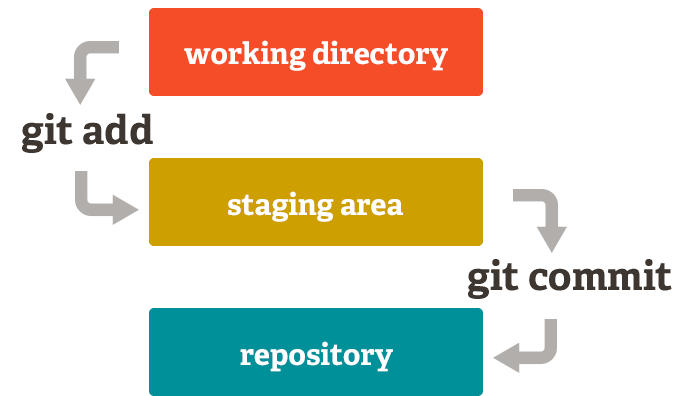
\includegraphics[width=0.75\textwidth]{img/file-status.png}
			\caption{Datei Status}
			\label{img:FileState}
		\end{figure}

	Was soll uns hier gezeigt werden? Das ist relativ einfach zu erklären. Wenn man Dateien im Arbeitsverzeichnis erstellt,
	weiß git noch nicht, das diese überhaupt existiert. Um Git Kenntnis zu verschaffen müssen die Datein in die \glqq 
	staging area\grqq. Wie das geht wird in der Abbildung \ref{img:FileState} auch schon beschrieben.
	Es reicht ein einfaches:
	
		\begin{lstlisting}[frame=single]
git add foo.tex
		\end{lstlisting}

	Erst jetzt weiß Git, dass die Datei \texttt{foo.tex} existiert. Wenn ihr jetzt einen \texttt{git status} macht,
	seht ihr, dass die Datei für einen Commit vorgemerkt ist. Das heißt allerdings auch, dass die entsprechende Datei
	noch nicht im Git-Repo ist.\par
	Um nun eine Datei in das Repo zu bringen muss die Datei committed werden. Wie der Abbildung \ref{img:FileState} zu
	entnehmen ist, maht ihr	das mit folgendem Befehl:

		\begin{lstlisting}[frame=single]
git commit -m "Your commit message"
		\end{lstlisting}

	Damit ist die Datei nun im Repo gelandet. Jetzt mag man sich die Frage stellen, warum es die Staging Area gibt.
	Warum commited man nicht einfach gleich? Die Staging Area kann man sich wie einen Zwischenstatus vorstellen.
	Hier kommen nur die Dateien rein, die auch committet werden sollen. Der Hintergrund ist, dass man keinen unfertigen
	Code im Repo hat.\par
	Wenn man gerade an einem Projekt arbeitet hat man auch die Möglichkeit alle Änderungen für den Commit forzubereiten.
	Dazu verwendet man diesen Befehl:

		\begin{lstlisting}[frame=single]
git add .
		\end{lstlisting}

	Danach braucht man nur noch einen \texttt{git commit} machen und alles ist festgehalten. Man sollte darauf achten, dass
	man beim \texttt{git add} und \texttt{git commit} immer den Kontext im Auge behält, um eine saubere Struktur zu 
	behalten. Es ist also am besten immer nur Sachen zu comitten, die auch in einem Zusammenhang stehen. Nochmal als
	Zusammenfassung die drei Status, die eine Datei haben kann: 
	

		\begin{enumerate}
			\item unstaged oder changed
			\item added und auf den commit wartend
			\item commited
		\end{enumerate}

	Bis jetzt ist alles was verändert wurde, nur bei euch lokal gemacht. Es hat noch keine Kommunikation nach außen
	stattgefunden. 

	\subsection{Das Remote Repo}
	Am Anfang des letzten Abschnittes habe ich es ja schon einmal kurz angerissen. Wir hatten schon Kontakt mit einem
	remote Repo. Das ist mit dem \texttt{git clone} passiert. Der Klon hat alle Informationen, die das Repo bis zu diesem
	Zeitpunkt hatte. Ein Klon ist also ein vollweriges Repository und hat auch schon einen remote Pfad zu GitHub.\par
	An dieser Stelle komme ich wieder zur Schuldokumentation. Mit dem Klon habt ihr die Verbindung zu meinem Repo schon.
	Das heißt, ihr könnt ganz einfach auf dem neusten Stand bleiben. Dazu gibt es zwei Befehle, die sich sehr ähnlich sind
	aber doch einen entscheidenden Unterschied haben. Hier erstmal die Befehle:

		\begin{lstlisting}[frame=single]
git fetch
git pull
		\end{lstlisting}

		\begin{itemize}
			\item \texttt{git fetch}: Dieser Befehl lädt die letzten Änderungen von meinem GitHub Repo herunter
				und bringt diese in \texttt{origin/master} unter. Euer Repo hat sich bis jetzt noch nicht
				verändert. Um euer Repo und meins auf den gleichen Stand zu bringen, müsst ihr die beiden Branch
				es\footnote{Entwicklungszweig} noch mergen\footnote{zusammenführen}. Wie das genau geht zeige
				ich euch in einem extra Abschnitt.
			\item \texttt{git pull}: Dieser Befehl macht \texttt{git fetch + git merge}. Der Vorteil liegt auf der
				Hand: Ihr braucht den merge nicht manuell machen. Allerdings ist auch Vorsicht geboten, da ihr
				in dem keine Kontrolle habt, was gemerged wird. Es wird ein simpler Rundumschlag gemacht.
		\end{itemize}

	Was ihr macht bleibt euch überlassen. Wenn es nur darum geht auf dem aktuellen Stand zu bleiben und ihr nicht 
	beabsichtigt Änderungen vorzunehmen, könnt ihr ruhig einen \texttt{git pull} machen. Grundsätzlich kann man sich merken
	das auf GitHub das Remote Repo liegt und jeder selbst ein lokales Repo hat.

	\subsection{Branching und Merging}
	\glqq Was zum Teufel soll das denn sein, bist du nicht bald mal fertig?\grqq\ Die Antwort kommt noch, keine Sorge.
	Branching und merging sind allerdings zwei essentielle Funktionen von git und nicht zu unterschätzen.
	Es ist vielleicht schon aufgefallen, dass ihr im Repo einen \glqq master\grqq\ Tag oder auch HEAD genannt habt.
	Dieser HEAD teilt euch mit in welchem Branch ihr euch befindet. Standardmäßg hat man einen, der eben \texttt{master}
	heißt. Hier eine Abbildung, um das Konzept einmal kurz darzustellen:

		\begin{figure}[H]
			\centering
			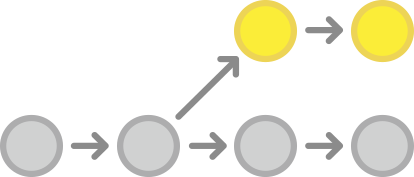
\includegraphics[width=0.75\textwidth]{img/branch.png}
			\caption{Branching}
			\label{img:branch}
		\end{figure}

	Was sagt uns das? Nehmen wir an, die grauen Punkte sind die \texttt{master} und die gelben Punkte die \texttt{feature1}
	commits. Wir sehen also zwei commits in der \texttt{master} Branch und dann wurde eine neue \texttt{feature1} erstellt.
	In der \texttt{feature1} Branch wurde dann ein weiterer Commit gemacht und in der \texttt{master} Branch wurden zwei 
	neue commits gemacht. Soweit so offensichtlich.\par
	Stellt sich erstmal die Frage, wie man eine neue Branch erstellt.

		\begin{lstlisting}[frame=single]
git branch feature1
		\end{lstlisting}

	Wenn ihr jetzt: 

		\begin{lstlisting}[frame=single]
git branch -v
		\end{lstlisting}

	seht ihr alle eure Brachnes. Demnach seht ihr jetzt die \texttt{master}- und die \texttt{feature1}-Branch.
	um in eine Branch zu wechseln nutzt ihr folgenden Befehl:

		\begin{lstlisting}[frame=single]
git checkout feature1
		\end{lstlisting}

	Was wird damit nun aber bewirkt. Ich habe vorhin von HEADERn gesprochen und eine Branch ist nichts anderes als ein
	solcher HEADER. Was das bewirkt seht ihr in Abbildung \ref{img:branch}. Die Commits werden in der Branch gemacht, in 
	der ihr euch gerade befindet. Damit könnt ihr also unabhängig von dem Hauptzweig (\texttt{master}) Arbeiten und
	experimentieren. Dabei wird allerdings keine Kopie der Branch erstellt. Hier kommt nämlich das Konzept der HEADER
	zum tragen. Je nach dem in welcher Branch ihr seid, verändert Git das Arbeitsverzeichnis, entsprechend der commits
	der jeweiligen Branch.\\[0.5cm]
	Um nun die Branches wieder zusammenzufügen, werden sie gemerged. Dabei ist zu beachten, dass immer die Branch verändert
	wird, in der ihr euch befindet. Angenommen ihr wollt \texttt{feature1} in \texttt{master} mergen:

		\begin{lstlisting}[frame=single]
git checkout master
git merge feature1
		\end{lstlisting}

	Und schon habt ihr die beiden Branches gemerged.

\section{The End}

Wer hier angekommen ist, hat ein Danke verdient. Wenn ihr jetzt noch wisst, warum ihr eigentlich angefangen habt dieses Dokument
zu lesen dürft ihr euch einen Keks nehmen.\par
Ich hoffe, ich konnte euch verständlich darlegen, wie unsere Schuldoku funktioniert und wie ihr sie nutzen könnt.
Wer noch Fragen oder Anregungen hat: Sagt mir bescheid. Wenn ihr Fehler gefunden habt, meldet euch.

\end{document}
